\begin{figure}[p]
\centering
\fbox{\parbox[c][4cm][c]{0.9\textwidth}{\centering Figure 1 pending}}
\caption{\textbf{The inferCNV workflow.} \todo{RESULT PENDING} Schematic of the expression model with heatmap snapshots from the 183-cell oligodendroglioma example data set (observations above, reference cells below; columns are genes ordered by genomic position). (a) Log-transformed counts after gene filtering and depth normalisation. (b) Residual expression after subtraction of the reference and smoothing along each chromosome. (c) After per-cell centering. (d) After the second reference subtraction, shown on the fold-change scale. (e) After denoising (\texttt{denoise\ =\ TRUE}). (f) i6 HMM state predictions per subcluster after Bayesian filtering, computed from the fold-change-scale residuals in (d) after subclustering. Panels (e) and (f) are alternative outputs derived from (d).}
\label{fig:1}
\end{figure}

\begin{figure}[p]
\centering
\fbox{\parbox[c][4cm][c]{0.9\textwidth}{\centering Figure 2 pending}}
\caption{\textbf{In-silico spike-in (h-spike) calibration of the HMM.} \todo{RESULT PENDING} (a) Mean--variance and (b) mean--dropout relationships of the reference cells with spline fits used to simulate counts. (c) Residual expression of the simulated h-spike chromosomes after the same processing as the real data, at relative copy number levels 0.01, 0.5, 1, 1.5, 2 and 3; the per-level distributions define the i6 emission parameters. (d) Comparison of i6 and i3 state calls on the same tumour.}
\label{fig:2}
\end{figure}

\begin{figure}[p]
\centering
\fbox{\parbox[c][4cm][c]{0.9\textwidth}{\centering Figure 3 pending}}
\caption{\textbf{inferCNV applied to tumours profiled with Smart-seq2.} \todo{RESULT PENDING} Residual expression heatmaps (top) and i6 HMM predictions with subclusters (bottom) for (a) oligodendroglioma, (b) glioblastoma, (c) melanoma and (d) H3K27M glioma. (e) \todo{or Supplementary Fig. S2} Synovial sarcoma: SS18--SSX fusion detection in cells classified as malignant or non-malignant by inferCNV.}
\label{fig:3}
\end{figure}

\begin{figure}[p]
\centering
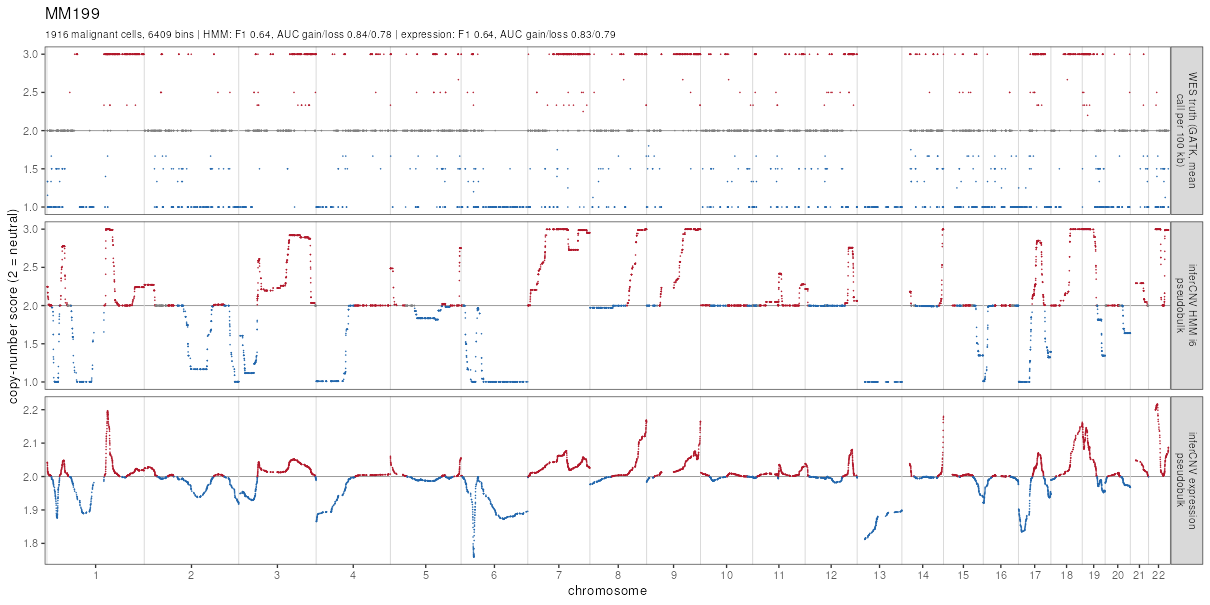
\includegraphics[width=\textwidth]{figures/fig4_MM199_genome.png}
\caption{\textbf{Comparison with DNA-based copy number in multiple myeloma MM199 (10x).} Top, whole-exome copy number segments (Schmid et al.~truth). Below, inferCNV pseudobulk scores over 1,916 malignant cells: HMM states after Bayesian filtering (CNV score) and final residual expression (expression score), in 100-kb bins along the genome. \todo{Panel with ROC curves and metric summary, if wanted; RESULT PENDING: BCH869 panel against WGS clone copy number.} Settings as in Methods.}
\label{fig:4}
\end{figure}

\begin{figure}[p]
\centering
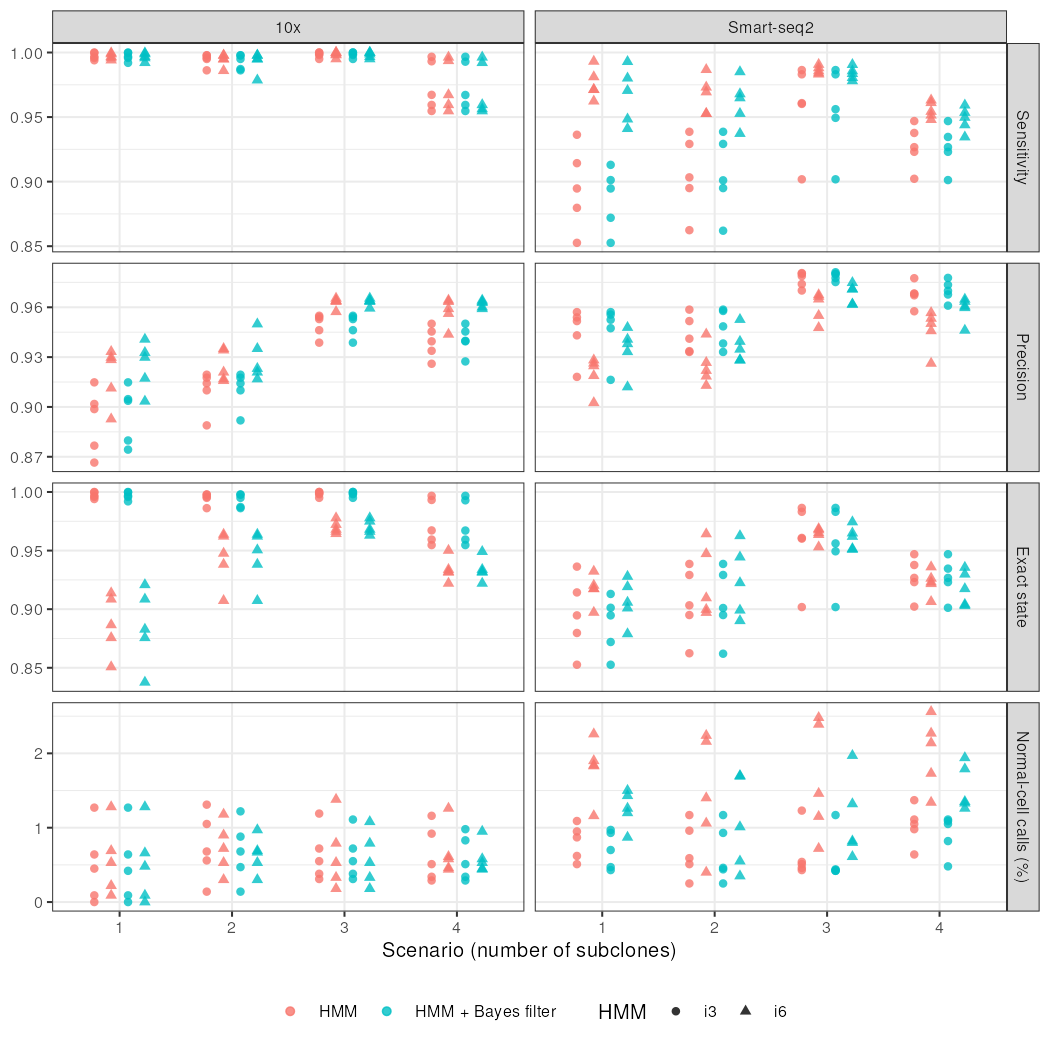
\includegraphics[width=\textwidth]{figures/fig5_simulation.png}
\caption{\textbf{Accuracy on simulated tumours.} Sensitivity, precision, exact-state accuracy, reference call rate and subcluster purity of the i6 HMM after Bayesian filtering for simulated 10x and Smart-seq2 data with one to four subclones (sim1--sim4), over five seeds (points) with means (bars); values in Table 1. \todo{Optional inset: i3 against i6.} \todo{Figure drawn from analyses/simulation/fig5\_simulation.png; check that it shows the master-build numbers of Table 1.}}
\label{fig:5}
\end{figure}

\begin{figure}[p]
\centering
\fbox{\parbox[c][4cm][c]{0.9\textwidth}{\centering Figure 6 pending}}
\caption{\textbf{Specificity and scale.} \todo{RESULT PENDING} (a) Non-neutral call rate in PBMC from healthy donors, by cell type, before and after Bayesian filtering. (b) Run time and peak memory against number of cells, with and without the Bayesian model and for i6 and i3.}
\label{fig:6}
\end{figure}

\begin{figure}[p]
\centering
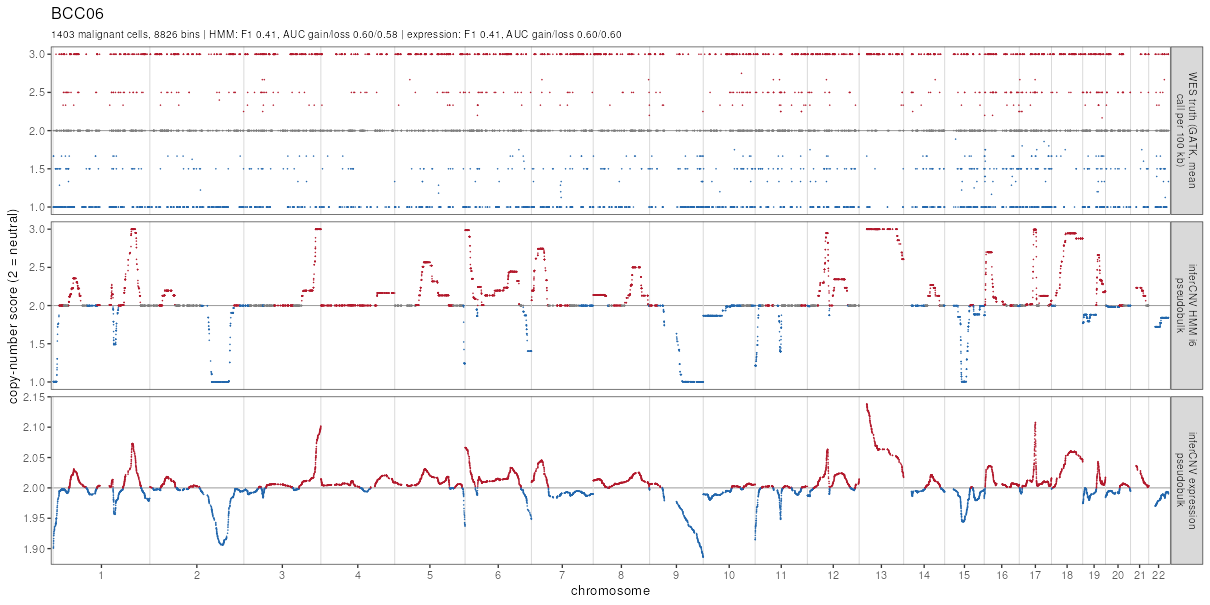
\includegraphics[width=\textwidth]{figures/figS1_BCC06_genome.png}
\caption{\textbf{Basal cell carcinoma BCC06 before and after treatment.} As Fig. 4, for BCC06 (1,403 malignant and 33 reference cells) and BCC06post (320 malignant and 280 reference cells). The exome segmentation of these samples is highly fragmented; see text.}
\label{fig:S1}
\end{figure}

% Supplementary Table S2: Metrics against DNA-based copy number.
% For each sample and score: number of malignant cells and bins, maximal F1, sensitivity and precision for gains and losses at the optimum, AUC and partial AUC for gains and losses, Pearson r; with the values reported by Schmid et al.~for inferCNV v1.10. (From analyses/fig4/metrics\_fig4.tsv and schmid2025\_reported\_infercnv\_v1.10.tsv.)
